
\documentclass[11pt,a4paper,slovene]{myarticle}

%Uporabljeni paketi
\usepackage[slovene]{babel}
\usepackage[utf8]{inputenc}
\usepackage{lmodern}
\usepackage[T1]{fontenc}
\usepackage{fancyhdr}
\usepackage{caption}
\captionsetup{font={default,footnotesize}, labelfont=bf, format=hang,indention=.0cm}
\usepackage{graphicx,epsfig}
\usepackage{amsmath}
\usepackage{multirow}
\usepackage{color}
\usepackage{url}
\usepackage{makeidx}
\usepackage[official]{eurosym}

\usepackage{hyperref}
\hypersetup{
   bookmarksnumbered=true,
   urlbordercolor={0 1 0},
   linkbordercolor={1 1 1},
   unicode=true,
   pdftitle={ Modeliranje Računalniških Omrežij },
   pdfauthor={Aljaž Markežič, Žan Valter Dragan},
   pdfdisplaydoctitle=true,
   pdftoolbar=true,
   pdfmenubar=true,
   pdfstartview=X Y Z
}

\urlstyle{same}

\setlength{\parskip}{12pt}
\setlength\parindent{0pt}
\setlength\unitlength{1mm}

\begin{document}
\label{naslov}
\pdfbookmark[1]{Naslov}{naslov}
\thispagestyle{empty}

\begin{center}
\begin{Large}
Modeliranje računalniških omrežij\\
Študijsko leto 2016/2017\\
\end{Large}

\vspace*{4cm}
\begin{LARGE}
\textbf{Implementacija IEEE 802.11 v orodju OMNeT++\\}
\end{LARGE}
\vspace*{0.5cm}

\begin{Large}
Modeliranje brezžičnih omrežij\\

\vspace*{4cm}

Aljaž Markežič, Žan Valter Dragan\\
Vpisna št. 63140157, 63140045\\

\vspace*{5cm}
Ljubljana, \today
\end{Large}
\end{center}

\pagebreak
\setcounter{page}{1}
\pagenumbering{arabic}


\label{Kazalo}
\pdfbookmark[1]{Kazalo}{Kazalo}
\tableofcontents
\thispagestyle{empty}
\pagebreak

\section{Uvod in motivacija}
V zadnjih letih se je zelo razširila nova doba povezljivosti, tako imenovani Internet of Things (IoT) oziroma Internet Stvari. Trg v omrežje povezanih naprav se neprestano povečuje z nezanemarljivo hitrostjo. Ker so kabli preokorni in Bluetooth ni vedno optimalen, se velikokrat išče rešitev v brezžičnih povezavah tipa IEEE 802.11. V tej seminarski nalogi se bova osredotočila na te povezave in jih nekaj tudi bolj nadrobno predstavila. Simulirala bova različna omrežja in preverila, kako se posemezen tip odnese. S tem bova pridobila podatke, kateri se nato lahko uporabijo pri izdelavi povezanih naprav.

\section{Opis specifikacij IEEE 802.11}
Zametki standarda IEEE 802.11 segajo že v leto 1985, vendar se je specifikacijo standardiziralo šele leta 1997. V 802.11 sta zajeti fizična plast ter del podatkovne plasti (Media Access Control - MAC). Standard se preko revizij spreminja še sedaj. Prva bolje zastopana različica je bila 802.11b, nekaj drugih pa je še a, g, n, ac, ... Ti standari delujejo na frekvencah 900MHz, 2.4GHz, 3.6GHz, 5GHz ter 60GHz. Naprave z 2.4GHz implementacijo občutijo občasne motnje drugih naprav, kot so mikrovalovne pečice, Bluetooth naprave in druge. Motnje rešujemo z raznimi modulacijami (Direct-Sequence Spread Spectrum, Orthogonal Frequency-Division Multiplexing). Povezave običajno dosegajo hitrosti v Mbit/s (od 1 do 866), kar pa so želeli spremeniti s standardom 802.11ad, kjer je možno doseči hitrosti do 7Gbit/s z uporabo višjih frekvenc.

\section{Uporabljene knjižnice}

\subsection{Razpoložljivi gradniki v OMNeT++}
\begin{itemize}
	\item \textbf{IPv4NetworkConfigurator:} modul, ki napravam v omrežju dodeli ipv4 naslove, ter skrbi za statično usmerjanje v omrežju. Modulu lahko nastavljamo naslednje atribute: address, netmask, multicast group, mtu,…
	\item \textbf{WirelessHost:} modul, ki simulira delovanje IP gostitelja (host-a), torej je sposoben posredovat, sprejemat in odgovarjat na sporočila, ki se pretakajo po omrežju. Nekaj od atributov ki jih lahko nastavljamo temu modulu so: bandwith,  transmiter.power, carierFrequency, reciever.sensiticity, antenaGain,…
	\item \textbf{Radio Medium:} modul, ki opisuje model deljenega fizičnega medija preko katerega potekajo vse komunikacije v omrežju. Modulu lahko določamo razne atribute kot so: material, backgroundNoise, pathloss, obstacleLoss,…, s pomočjo katerih lahko simuliramo dejanski medij preko katerih bi potekala brezžična povezava
	\item \textbf{PhysicalEnvironment:} modul, ki simulira fizične ovire, ki se lahko znajdejo v testnem okolju. S pomočjo tega modula lahko simuliramo kako se bo odzivalo omrežje, saj fizične ovire vplivajo na porabo energije, ter premikanje brezžičnih gostiteljev (wirelessHosts). Modulu lahko nastavljamo naslednje atribute: position, orientation, shape, material, color, opacity
	\item \textbf{AccessPoint:} modul, ki simulira generično vstopno točko (access point), preko katere si lahko naprave izmenjujejo sporočila, ter podpira več brezžičnih frekvenc in ethernet vhodov.
\end{itemize}

\subsection{Zgledi omrežij 802.11 v OMNeT++}
Za delo v okolju OMNeT++ imamo na voljo kar nekaj primerov, med katerimi je tudi ogrodje INET. Ti primeri služija koz prikaz možnih postavitev, kot tudi morebitnih težav, ki se lahko pojavijo znotraj tovrstnih omrežij. V nadaljevanju so predstavljeni trije primeri brezžičnih omrežij.
\subsubsection{Primer1 - LAN 802.11}
Omrežje je definirano v datoteki Lan80211.ned v kateri je predstavljeno omrežje za testiranje 802.11 modela v infrastrukturnem načinu. Omrežje je sestavljeno iz vstopne točke (Access Point – AP) v infrastrukturnem načinu, ter poljubnim številom gostiteljev(host) tipa 	WirelessHost. Konfiguracija omrežja je opisana v datoteki omnetpp.ini v katerem lahko definiramo razne atribute omržeja, kot so: constraintArea(območje kritja AP), MAC naslov AP, gibanje gostiteljev, ... Simulacija (1*AP, 2*HOST) poteka tako, da prvo host[1] pošlje arpReq AP kjer zahteva MAC address za določen IP, AP na sprejeto sporočilo odgovori z ACK, ter nato broadcasta ta arpReq vsem ostalim napravam v območju kritja. Ko ciljna naprava dobi ARPReq, pošlje AP nazaj ARPReply, ta pa mu nazaj odgovori z ACK. Potem AP broadcasta 	ARPReply vsem napravam v dosegu. Ko ciljna naprava dobi paket odgovori nazaj z ACK, kar pomeni da sedaj host[1], ve MAC naslov naprave za IP naslov, ki ga je zahteval v ARPReq. Tako se lahko začne komunikaciaj med host[1] pa host[0], kar je v simulaciji izvedeno preko ICMP ping paketov.
\begin{figure}[h]
	\centering
		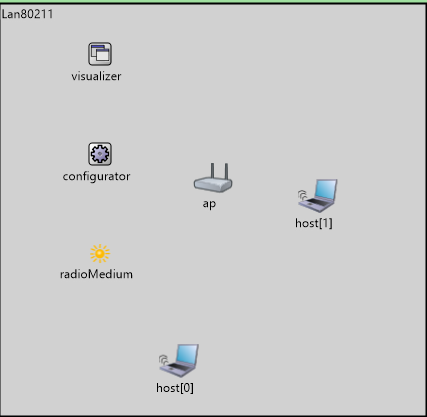
\includegraphics[width=0.9\textwidth, keepaspectratio=true]{./images/lan80211.png}
	\caption{LAN 802.11}
	\label{fig:lan80211}
\end{figure}

\subsubsection{Primer2 - QOS}
Omrežje je definirano v datoteki Throughput.ned v kateri je predstavljeno omrežje, ki simulira celotno vzpostavitev povezazve med gostiteljem(hostom), ter strežnikom(server), ki sta oba tipa WirelessHost preko vstopne točke (Access Pointa – AP), ki je tipa AccessPoint. Konfiguracija omrežje je opisana v datoteki omnetpp.ini kjer lahko spreminjamo iste paramtere kot v prejšnjem primeru, torej: constraintArea(območje kritja AP), MAC naslov AP, ... Simulacija se začne tako da AP pošilja Beacon pakete s katerimi se oglašuje, oziroma poziva naprave da se povežejo nanj. Če se naprave želijo povezati na AP to storijo Probe Request paketom, na kar AP 	odgovori z Probe response paketom. Nato so začne faza avtentikacije, asociacije in ARP discovery faza, kjer si AP in gostiteljske naprave izmenjenajo razne podatke za vzpostavitev povezave. Ko je gostiteljska naprava dokončno vzpostavila povezavo z AP, se začne komunikacija med strežnikom in odjemalcem, kjer odjemalec zahteva različne pakete kot so, Video, WWW, FTP, ...
\begin{figure}[h]
	\centering
		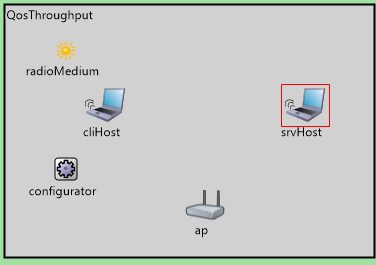
\includegraphics[width=0.9\textwidth, keepaspectratio=true]{./images/qos.png}
	\caption{QOS}
	\label{fig:QOS}
\end{figure}

\subsubsection{Primer3 - Synchronized}
Ta primer prikaže morebitne napake, katere se pojavijo ob sinhronem oddajanju signalov večih naprav znotraj brezžičnega omrežja. Na voljo imamo sledeča gradnika: radioMedium in node. Naprave oddajajo UDP pakete v ad hoc omrežje sinhrono - vedno pošiljajo ob istem času. Le-to povzroči izgubo paketov zaradi medsebojnih motenj valovanj. To razrešimo z vpeljavo naključnih zakasnitev na aplikacijski ravni, kar pomeni, da omrežje postane asinhrono.
\begin{figure}[h]
	\centering
		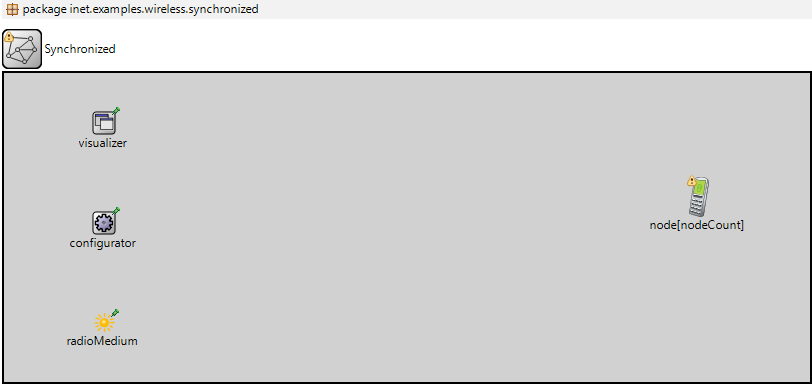
\includegraphics[width=0.9\textwidth, keepaspectratio=true]{./images/syn-components.png}
	\caption{Synchronized - Gradniki}
	\label{fig:synchronizedgradniki}
\end{figure}

V simulacijskih nastavitvah je možno nastaviti število naprav (privzeta vrednost je 30), ter območje znotraj katerega se nahajajo. Na voljo sta tudi dve konfiguraciji - sinhrona in asinhrona, kjer nastavimo čas pošiljanja paketov. Pri asinhroni konfiguraciji je na voljo tudi nastavitev tipa MAC naslova, katera pa je privzeto zakomentirana.
\begin{figure}[h]
	\centering
		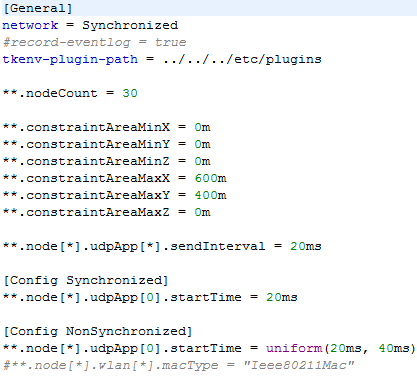
\includegraphics[width=0.9\textwidth, keepaspectratio=true]{./images/syn-settings.png}
	\caption{Synchronized - Nastavitve Simulacije}
	\label{fig:synchronizednastavitvesimulacije}
\end{figure}
\begin{figure}[h]
	\centering
		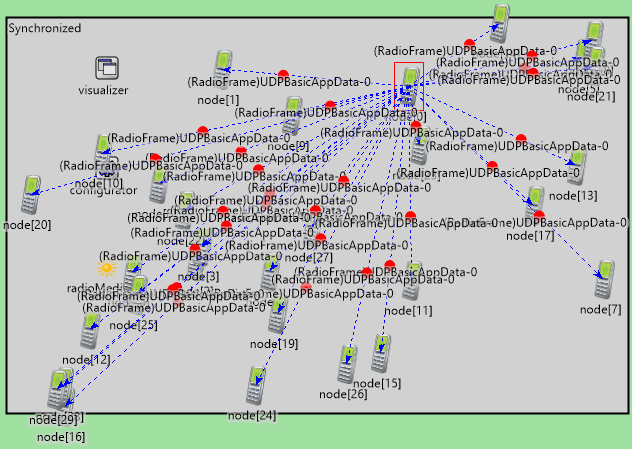
\includegraphics[width=0.9\textwidth, keepaspectratio=true]{./images/syn-simulation.png}
	\caption{Synchronized - Simulacija}
	\label{fig:synchronizedsimulacija}
\end{figure}

\section{Rešitev}
Podroben opis rešitve. Sem spadajo načrtovanje, struktura omrežja, opis sprogramiranih modulov in omrežij.

\section{Simulacije in rezultati}
Podroben opis simulacijskega algoritma, rezultati in pregled grafov performančne analize.

\section{Zaključek}
Ali ste izpolnili cilje in možne nadaljne nadgradnje. Pri samem opisu rešitve se običajno sklicujemo na reference, npr. \cite{omnetpp}. 

\pagebreak
\bibliographystyle{plain}
\bibliography{references}

\end{document}







